% p5.tex (Расширенная версия)

\examquestion{21}{Интеграл с переменным верхним пределом и его непрерывность}
{Сформулируйте и докажите теорему о непрерывности функции $\Phi(x) = \int_a^x f(t)dt$ на сегменте $[a, b]$, предполагая лишь ограниченность и интегрируемость исходной функции $f(t)$.}

\paragraph{Суть на пальцах}
Интеграл с переменным верхним пределом $\Phi(x)$ - это накопленная площадь под графиком от старта $a$ до текущей точки $x$. Если мы чуть-чуть сдвинем границу $x$ на шаг $\Delta x$, к нашей площади добавится только очень тонкая вертикальная полоска. Так как исходная функция ограничена (не улетает в бесконечность), площадь этой узкой полоски будет стремиться к нулю. Площадь меняется плавно, без телепортов и скачков. Это и есть непрерывность.

\paragraph{Формулировка}
Пусть $f(t)$ интегрируема на $[a, b]$. Следовательно, она ограничена на нем: существует число $M > 0$ такое, что $|f(t)| \le M$ для всех $t \in [a, b]$.
Теорема: функция $\Phi(x) = \int_a^x f(t)dt$ непрерывна в любой точке $x \in [a, b]$.

\begin{proof}
1. Зафиксируем точку $x$ и дадим ей малое приращение $\Delta x$.
2. Запишем приращение функции $\Phi$:
$$ \Delta \Phi = \Phi(x+\Delta x) - \Phi(x) = \int_a^{x+\Delta x} f(t)dt - \int_a^x f(t)dt $$
3. По свойству аддитивности интеграла (разбиение отрезка интегрирования), разность этих двух интегралов дает интеграл по маленькому кусочку от $x$ до $x+\Delta x$:
$$ \Delta \Phi = \int_x^{x+\Delta x} f(t)dt $$
4. Оценим модуль этого приращения, используя свойство $| \int \dots | \le \int | \dots |$:
$$ |\Delta \Phi| = \left| \int_x^{x+\Delta x} f(t)dt \right| \le \left| \int_x^{x+\Delta x} |f(t)| dt \right| $$
5. Так как функция ограничена ($|f(t)| \le M$), заменим подынтегральное выражение на максимум:
$$ |\Delta \Phi| \le \left| \int_x^{x+\Delta x} M dt \right| = M \cdot |(x+\Delta x) - x| = M \cdot |\Delta x| $$
6. Переходим к пределу при $\Delta x \to 0$. Константа $M$ фиксирована, поэтому $M \cdot |\Delta x|$ стремится к нулю.
$$ \lim_{\Delta x \to 0} \Delta \Phi = 0 $$
Приращение функции стремится к нулю при стремлении приращения аргумента к нулю. Непрерывность доказана.
\end{proof}


% --- Для Вопроса 21 (Интеграл с переменным верхним пределом) ---
\begin{tcolorbox}[colback=gray!5, colframe=black, boxrule=0.5pt, arc=0pt]
\textbf{Резюмируем:} \\
\textbf{Тезис:} Функция $\Phi(x) = \int_a^x f(t)dt$ непрерывна, если $f(t)$ ограничена ($|f| \le M$). \\
\textbf{Ход:} Записываем приращение $\Delta \Phi = \int_a^{x+\Delta x} - \int_a^x = \int_x^{x+\Delta x} f(t)dt$. \\
\textbf{Трюк:} Оцениваем модуль: $|\Delta \Phi| \le \int_x^{x+\Delta x} |f(t)| dt \le M \cdot |\Delta x|$. \\
\textbf{Финал:} При $\Delta x \to 0$ получаем $M|\Delta x| \to 0 \implies \lim \Delta \Phi = 0$. Непрерывность доказана.
\end{tcolorbox}

% -----------------------------------------------------

\examquestion{22}{Теорема Барроу о производной интеграла по верхнему пределу}
{Сформулируйте и проведите доказательство теоремы Барроу. Покажите, как из приращения $\Delta\Phi$ с помощью первой теоремы о среднем значении выделяется значение функции в промежуточной точке. Обоснуйте важность непрерывности.}

\paragraph{Суть на пальцах}
Если $\Phi(x)$ - это площадь, то производная $\Phi'(x)$ - это скорость, с которой эта площадь растет при движении вправо. Логично, что чем выше график функции $f(x)$ в конкретной точке, тем быстрее прирастает площадь. Теорема Барроу это строго доказывает: скорость роста площади в точке $x$ в точности равна значению самой функции в этой точке. 

\paragraph{Формулировка}
Если функция $f(t)$ интегрируема на $[a, b]$ и непрерывна в конкретной точке $x \in [a, b]$, то функция $\Phi(x) = \int_a^x f(t)dt$ дифференцируема в этой точке, и ее производная равна $\Phi'(x) = f(x)$.

\begin{proof}
1. Берем приращение интеграла (как в прошлом билете):
$$ \Delta \Phi = \int_x^{x+\Delta x} f(t)dt $$
2. Применяем первую теорему о среднем (где весовая функция $g(t) = 1$). По теореме существует такая точка $\xi$ между $x$ и $x+\Delta x$, что интеграл равен площади прямоугольника с высотой $f(\xi)$ и шириной $\Delta x$:
$$ \Delta \Phi = f(\xi) \cdot \Delta x $$
3. Подставляем это в классическое определение производной:
$$ \Phi'(x) = \lim_{\Delta x \to 0} \frac{\Delta \Phi}{\Delta x} = \lim_{\Delta x \to 0} \frac{f(\xi) \cdot \Delta x}{\Delta x} = \lim_{\Delta x \to 0} f(\xi) $$
4. Обоснование роли непрерывности: точка $\xi$ зажата на отрезке между $x$ и $x+\Delta x$. Когда $\Delta x \to 0$, этот отрезок стягивается в точку, и $\xi$ вынуждена стремиться к $x$. Но мы имеем право написать, что $\lim_{\xi \to x} f(\xi) = f(x)$ ТОЛЬКО при условии, что функция $f(t)$ непрерывна в точке $x$. Без непрерывности предел мог бы не существовать или не равняться значению функции, и вся логика бы рухнула.
5. Итог: $\Phi'(x) = f(x)$.
\end{proof}

% --- Для Вопроса 22 (Теорема Барроу) ---
\begin{tcolorbox}[colback=gray!5, colframe=black, boxrule=0.5pt, arc=0pt]
\textbf{Резюмируем:} \\
\textbf{Тезис:} Если $f(t)$ непрерывна в $x$, то $\Phi'(x) = f(x)$. Скорость роста площади равна функции. \\
\textbf{Ход:} Приращение $\Delta \Phi = \int_x^{x+\Delta x} f(t)dt$. По 1-й теореме о среднем $\Delta \Phi = f(\xi)\Delta x$, где $\xi \in [x, x+\Delta x]$. \\
\textbf{Трюк:} Ищем производную: $\Phi'(x) = \lim_{\Delta x \to 0} \frac{f(\xi)\Delta x}{\Delta x} = \lim_{\Delta x \to 0} f(\xi)$. \\
\textbf{Финал:} При $\Delta x \to 0$ отрезок стягивается, $\xi \to x$. Из-за непрерывности $\lim f(\xi) = f(x)$. Итог: $\Phi'(x) = f(x)$.
\end{tcolorbox}


% --- Вопрос 23 ---
\examquestion{23}{Приложение теоремы Барроу к вычислению пределов}
{Сформулируйте и обоснуйте метод раскрытия неопределенностей вида 0/0 и $\infty/\infty$ по правилу Лопиталя для функций, содержащих интегралы с переменными пределами.}

\paragraph{Суть на пальцах}
Бывает, что в пределе торчит интеграл, границы которого зависят от $x$. Считать его в лоб — плохая идея. Но если при подстановке мы получаем неопределенность $0/0$ или $\infty/\infty$, правило Лопиталя разрешает взять производные от числителя и знаменателя. 

Вся фишка в том, как продифференцировать такой интеграл. Мы "вставляем" границы внутрь функции и домножаем на их собственные производные.

\paragraph{Формулировка метода}
Пусть нам нужно найти предел $\lim_{x \to x_0} \frac{F(x)}{g(x)}$, где числитель (или знаменатель) имеет вид $F(x) = \int_{a(x)}^{b(x)} f(t)dt$.
По правилу Лопиталя мы переходим к пределу отношения производных: $\lim_{x \to x_0} \frac{F'(x)}{g'(x)}$.
Производная интеграла считается строго по формуле Лейбница:
$$ F'(x) = \frac{d}{dx} \left( \int_{a(x)}^{b(x)} f(t)dt \right) = f(b(x)) \cdot b'(x) - f(a(x)) \cdot a'(x) $$

\paragraph{Логическое обоснование формулы}
Вывод формулы строится на трех последовательных шагах:
1. \textbf{Базовый случай (Барроу):} Если меняется только верхний предел, то по теореме Барроу производная равна самой функции: $\frac{d}{dx} \int_a^x f(t)dt = f(x)$.
2. \textbf{Сложная функция:} Если сверху стоит не голый $x$, а функция $b(x)$, то по правилу дифференцирования сложной функции берем производную "внешней" части (интеграла) и умножаем на производную "внутренней" (самой границы): $\frac{d}{dx} \int_a^{b(x)} f(t)dt = f(b(x)) \cdot b'(x)$.
3. \textbf{Две переменные границы:} Разделяем интеграл фиксированной точкой $C \in (a, b)$ и переворачиваем нижний предел:
$$ \int_{a(x)}^{b(x)} f(t)dt = \int_{a(x)}^C f(t)dt + \int_C^{b(x)} f(t)dt = \int_C^{b(x)} f(t)dt - \int_C^{a(x)} f(t)dt $$
Дифференцируя полученную разность по правилу сложной функции, получаем финальную формулу.

\paragraph{Условия применимости}
Чтобы метод сработал законно, нужно проверить 5 вещей:
1. Тип неопределенности строго $0/0$ или $\infty/\infty$.
2. Пределы интегрирования $a(x)$ и $b(x)$ дифференцируемы возле $x_0$.
3. Знаменатель не равен нулю: $g'(x) \neq 0$ в проколотой окрестности $x_0$.
4. Подынтегральная функция $f(t)$ непрерывна. Иначе Барроу сломается.
5. Предел отношения производных реально существует.

\paragraph{Практический пример}
Найдем предел:
$$ \lim_{x \to 0} \frac{\int_0^{x^2} \sin(\sqrt{t}) dt}{x^3} $$

1. \textbf{Проверка:} При $x \to 0$ интеграл идет от 0 до 0 (дает 0), знаменатель тоже 0. Имеем $0/0$, Лопиталь разрешен.
2. \textbf{Дифференцирование:} Знаменатель: $(x^3)' = 3x^2$. Числитель дифференцируем по нашей формуле (нижний предел — константа, его производная 0):
$$ \frac{d}{dx} \int_0^{x^2} \sin(\sqrt{t}) dt = \sin(\sqrt{x^2}) \cdot (x^2)' = \sin(|x|) \cdot 2x \xrightarrow{x \to 0^+} 2x \sin(x) $$
3. \textbf{Вычисление предела:} Собираем отношение производных и используем первый замечательный предел ($\frac{\sin(x)}{x} \to 1$):
$$ \lim_{x \to 0} \frac{2x \sin(x)}{3x^2} = \lim_{x \to 0} \left( \frac{2}{3} \cdot \frac{\sin(x)}{x} \right) = \frac{2}{3} \cdot 1 = \frac{2}{3} $$
% --- Для Вопроса 23 (Лопиталь и Барроу) ---
\begin{tcolorbox}[colback=gray!5, colframe=black, boxrule=0.5pt, arc=0pt]
\textbf{Резюмируем:} \\
\textbf{Тезис:} Раскрытие $0/0$ через Лопиталя с производной интеграла $F'(x) = f(b(x))b'(x) - f(a(x))a'(x)$. \\
\textbf{Ход:} Интеграл $\int_{a(x)}^{b(x)}$ разбиваем точкой $C$ на два куска: $\int_C^{b(x)} - \int_C^{a(x)}$. \\
\textbf{Трюк:} По правилу сложной функции берем производную: внешняя (Барроу) на внутреннюю (производная границы). \\
\textbf{Финал:} Проверяем $0/0$, непрерывность $f(t)$, производную знаменателя $\neq 0$. Подставляем Лейбница в предел отношения производных.
\end{tcolorbox}



\examquestion{24}{Теорема Ньютона-Лейбница}
{Сформулируйте и докажите основную теорему интегрального исчисления для функции $f(x) \in C[a, b]$. Опишите решение главной проблемы интеграла Римана.}

\paragraph{Суть на пальцах}
Главная проблема интеграла Римана - это процесс его вычисления. Резать фигуру на бесконечное число столбиков, составлять гигантские суммы и брать от них предел - это адски сложно. Теорема Ньютона-Лейбница - это фундаментальный читкод матанализа. Она говорит: забудь про суммы. Просто найди первообразную (функцию, которая при дифференцировании дает $f(x)$) и вычти ее значение на старте из значения на финише. Всё.

\paragraph{Формулировка}
Если функция $f(x)$ непрерывна на отрезке $[a, b]$, а $F(x)$ - любая ее первообразная на этом отрезке (то есть $F'(x) = f(x)$), то справедлива формула:
$$ \int_a^b f(x)dx = F(b) - F(a) $$

\begin{proof}
1. По теореме Барроу мы знаем, что интеграл с переменным верхним пределом $\Phi(x) = \int_a^x f(t)dt$ дифференцируем и $\Phi'(x) = f(x)$. Значит, $\Phi(x)$ - это одна из возможных первообразных для нашей функции.
2. Из дифференциального исчисления известно, что любые две первообразные одной и той же функции отличаются друг от друга максимум на константу $C$.
3. Значит, любую абстрактную первообразную $F(x)$ можно выразить через наш интеграл:
$$ F(x) = \Phi(x) + C = \int_a^x f(t)dt + C $$
4. Чтобы найти точное значение $C$, подставим в это уравнение $x = a$. Интеграл от $a$ до $a$ равен нулю (площадь нулевой ширины):
$$ F(a) = \int_a^a f(t)dt + C = 0 + C \implies C = F(a) $$
5. Теперь подставим в уравнение конец отрезка $x = b$:
$$ F(b) = \int_a^b f(t)dt + F(a) $$
6. Переносим $F(a)$ в левую часть и переписываем интеграл (буква переменной интегрирования $t$ не важна, меняем на привычный $x$):
$$ \int_a^b f(x)dx = F(b) - F(a) $$
Теорема доказана.
\end{proof}

% --- Для Вопроса 24 (Теорема Ньютона-Лейбница) ---
\begin{tcolorbox}[colback=gray!5, colframe=black, boxrule=0.5pt, arc=0pt]
\textbf{Резюмируем:} \\
\textbf{Тезис:} Основная теорема матанализа: $\int_a^b f(x)dx = F(b) - F(a)$. \\
\textbf{Ход:} По Барроу $\Phi(x) = \int_a^x f(t)dt$ — это одна из первообразных. Любая другая $F(x) = \Phi(x) + C$. \\
\textbf{Трюк:} Подставляем $x = a$: $F(a) = \int_a^a f(t)dt + C = 0 + C \implies C = F(a)$. \\
\textbf{Финал:} Подставляем $x = b$: $F(b) = \int_a^b f(t)dt + F(a)$. Переносим $F(a)$ и получаем готовую формулу.
\end{tcolorbox}


% --- Вопрос 25 ---
\examquestion{25}{Вычисление площади в полярных координатах}
{Сформулируйте задачу о нахождении площади криволинейного сектора. Строго выведите формулу площади $S(D) = \frac{1}{2} \int_{\alpha}^{\beta} \rho^2(\varphi) d\varphi$ для непрерывной функции $\rho(\varphi) \ge 0$, используя аппарат верхних и нижних сумм Дарбу, свойство квадрируемости и теорему Кантора о равномерной непрерывности.}

\paragraph{Суть на пальцах}
В декартовых координатах мы резали площадь на вертикальные прямоугольные столбики ($dS = f(x)dx$). В полярных координатах мы режем фигуру лучами из начала координат на тонкие «кусочки пиццы». 
Каждый такой кусочек мы зажимаем между двумя идеальными круговыми секторами: один чуть поменьше (радиуса $m_k$, сидит целиком внутри), другой чуть побольше (радиуса $M_k$, вылезает наружу). Площадь кругового сектора из школы равна $\frac{1}{2}R^2 \Delta \varphi$. 
Суммируя маленькие секторы, получаем нижнюю площадь (нижнюю сумму Дарбу), а суммируя большие — верхнюю. При измельчении угла разбиения эти площади схлопываются в один определенный интеграл. Это схлопывание и доказывает квадрируемость (существование площади).

\paragraph{1. Постановка задачи}
Пусть на отрезке $[\alpha, \beta]$ задана непрерывная функция $\rho(\varphi) \ge 0$. Фигура $D$, ограниченная лучами $\varphi = \alpha$, $\varphi = \beta$ и кривой $\rho = \rho(\varphi)$, называется \textbf{криволинейным сектором}. Задача — доказать, что у фигуры $D$ есть площадь (она квадрируема), и найти её.
\paragraph{Геометрический смысл зажатия секторов}
\begin{center}
\begin{tikzpicture}[scale=1.4]
    % Оси
    \draw[->, thick, gray] (0,0) -- (4,0) node[right, black] {$x$};
    
    % Границы сектора (лучи \alpha и \beta)
    \draw[thick, dashed] (0,0) -- (25:3.8) node[right] {$\varphi = \alpha$};
    \draw[thick, dashed] (0,0) -- (70:3.5) node[above] {$\varphi = \beta$};
    
    % Реальная кривая \rho(\varphi)
    \draw[ultra thick, blue, domain=25:70, samples=100] plot (\x,{2.5 + 0.5*sin(\x*3)}) node[above right] {$\rho(\varphi)$};
    
    % Выделенный частичный сектор \Delta \varphi_k
    \draw[gray, thin] (0,0) -- (40:3.5);
    \draw[gray, thin] (0,0) -- (55:3.5);
    \node at (47:1.2) {$\Delta\varphi_k$};
    
    % Вписанный круговой сектор (Нижняя сумма Дарбу, радиус m_k)
    \draw[red, thick, fill=red!10, opacity=0.7] (0,0) -- (40:2.15) arc (40:55:2.15) -- cycle;
    \node[red, below right] at (45:2.15) {$m_k$};
    
    % Описанный круговой сектор (Верхняя сумма Дарбу, радиус M_k)
    \draw[green!60!black, thick] (40:2.95) arc (40:55:2.95);
    \draw[green!60!black, dashed] (0,0) -- (40:2.95);
    \draw[green!60!black, dashed] (0,0) -- (55:2.95);
    \node[green!60!black, above right] at (50:2.95) {$M_k$};
    
    % Кусок реальной кривой внутри этого шага
    \draw[ultra thick, blue, domain=40:55] plot (\x,{2.5 + 0.5*sin(\x*3)});
    
    \node[below left] at (0,0) {$O$};
\end{tikzpicture}
\end{center}

\begin{figure}[h!]
    \centering
    \begin{center}
        Примерно вот так выглядят секторы $M_k$ и $m_k$:
    \end{center}
    \vspace{0.5em}
    \begin{minipage}{0.45\textwidth}
        \centering
        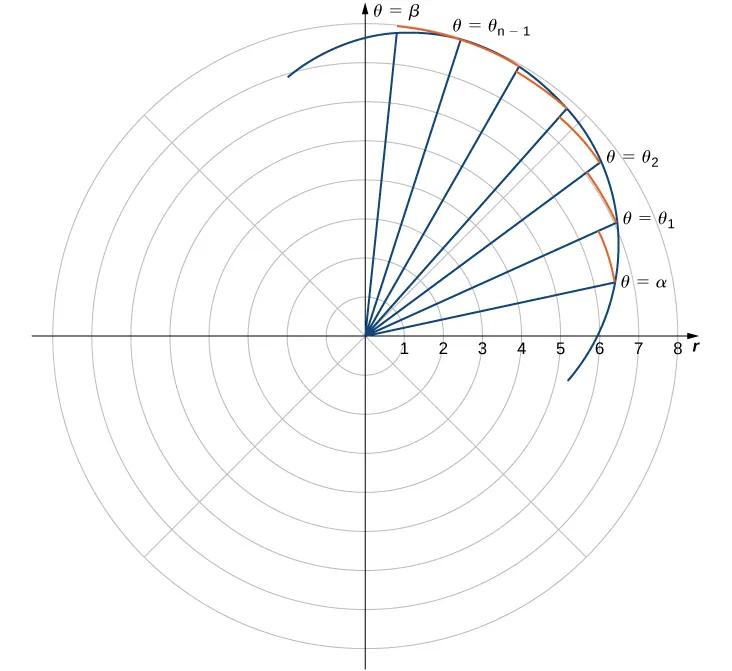
\includegraphics[width=\textwidth]{m_low.png}
        \caption{Нижняя грань $m_k$}
    \end{minipage}
    \hfill
    \begin{minipage}{0.45\textwidth}
        \centering
        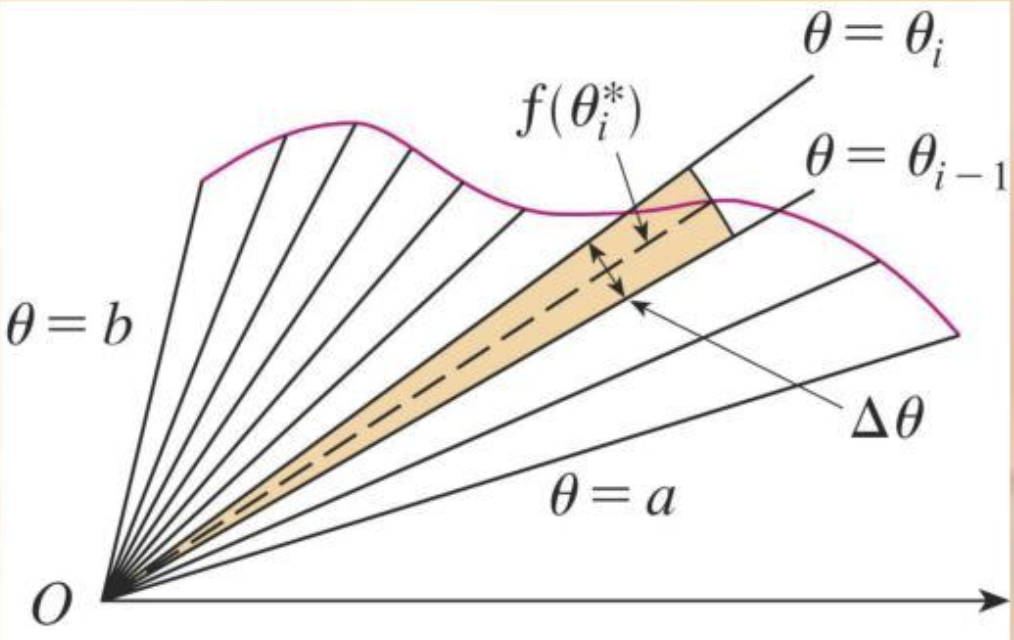
\includegraphics[width=\textwidth]{m_up.png}
        \caption{Верхняя грань $M_k$}
    \end{minipage}
\end{figure}

\paragraph{2. Построение сумм Дарбу}
1. Разобьем отрезок $[\alpha, \beta]$ точками $\alpha = \varphi_0 < \varphi_1 < \dots < \varphi_n = \beta$ на $n$ частей с шагом $\Delta \varphi_k = \varphi_k - \varphi_{k-1}$.
2. Функция $\rho(\varphi)$ непрерывна на компакте, значит, по теореме Вейерштрасса на каждом кусочке она достигает минимума $m_k$ и максимума $M_k$.
3. Составим нижнюю $s(T)$ и верхнюю $S(T)$ суммы Дарбу (складываем площади школьных круговых секторов):
$$ s(T) = \sum_{k=1}^n \frac{1}{2} m_k^2 \Delta \varphi_k, \quad S(T) = \sum_{k=1}^n \frac{1}{2} M_k^2 \Delta \varphi_k $$
По свойству монотонности площади, истинная площадь $S(D)$ обязана лежать между ними: $s(T) \le S(D) \le S(T)$.

\paragraph{3. Доказательство квадрируемости (т.е. имеет площадь)}
\begin{proof}
Фигура квадрируема, если разность верхней и нижней сумм стремится к нулю при мелкости разбиения $\lambda \to 0$. Распишем эту разность:
$$ S(T) - s(T) = \frac{1}{2} \sum_{k=1}^n (M_k^2 - m_k^2) \Delta \varphi_k = \frac{1}{2} \sum_{k=1}^n (M_k - m_k)(M_k + m_k) \Delta \varphi_k $$

Оценим множители:
1. Так как $\rho(\varphi)$ непрерывна на $[\alpha, \beta]$, она ограничена некоторой константой $C$, то есть $\rho(\varphi) \le C$. Значит, $(M_k + m_k) \le 2C$.
2. По \textbf{теореме Кантора}, непрерывная на отрезке функция является равномерно непрерывной. Это значит, что для любого $\varepsilon > 0$ можно выбрать настолько мелкое разбиение, что колебание функции на каждом кусочке станет меньше $\varepsilon$: $(M_k - m_k) < \varepsilon$.

Подставим эти оценки в разность сумм:
$$ S(T) - s(T) \le \frac{1}{2} \sum_{k=1}^n \varepsilon \cdot 2C \cdot \Delta \varphi_k = \varepsilon C \sum_{k=1}^n \Delta \varphi_k $$
Так как сумма всех углов $\sum \Delta \varphi_k = \beta - \alpha$ (полный угол сектора), получаем:
$$ S(T) - s(T) \le \varepsilon C (\beta - \alpha) $$
При мелкости разбиения $\lambda \to 0$ шаг $\varepsilon \to 0$, следовательно:
$$ \lim_{\lambda \to 0} (S(T) - s(T)) = 0 $$
Верхняя и нижняя суммы Дарбу сошлись к одному числу. Это доказывает, что верхний и нижний интегралы Дарбу равны, функция площади существует, а сама фигура $D$ по определению \textbf{квадрируема}.
\end{proof}

\paragraph{4. Вывод финальной формулы}
Построенные суммы $s(T)$ и $S(T)$ являются точными суммами Дарбу для функции $f(\varphi) = \frac{1}{2}\rho^2(\varphi)$. Так как $\rho(\varphi)$ непрерывна, то и $f(\varphi)$ непрерывна, а значит — интегрируема по Риману.
Предел сумм Дарбу при $\lambda \to 0$ равен определенному интегралу:
$$ S(D) = \int_{\alpha}^{\beta} \frac{1}{2} \rho^2(\varphi) d\varphi $$
Выносим константу $\frac{1}{2}$ за знак интеграла:
$$ S(D) = \frac{1}{2} \int_{\alpha}^{\beta} \rho^2(\varphi) d\varphi $$

% --- Для Вопроса 25 (Вычисление площади в полярных координатах) ---
\begin{tcolorbox}[colback=gray!5, colframe=black, boxrule=0.5pt, arc=0pt]
\textbf{Резюмируем:} \\
\textbf{Тезис:} Криволинейный сектор квадрируем, его площадь $S = \frac{1}{2} \int_{\alpha}^{\beta} \rho^2(\varphi) d\varphi$. \\
\textbf{Ход:} Разбиваем угол. Зажимаем площадь между круговыми секторами с $m_k$ и $M_k$. Разность $S(T) - s(T) = \frac{1}{2} \sum (M_k - m_k)(M_k + m_k) \Delta \varphi_k$. \\
\textbf{Трюк:} Ограниченность дает $(M_k + m_k) \le 2C$. Равномерная непрерывность (Кантор) дает колебание $(M_k - m_k) < \varepsilon$. \\
\textbf{Финал:} Оценка разности $\le \varepsilon C (\beta - \alpha) \to 0$. Суммы сошлись, предел равен интегралу от $\frac{1}{2}\rho^2(\varphi)$.
\end{tcolorbox}